\appendix

\chapter{Amazon Athena } \label{athena-appendix}

\section{Création de la table traceroutes } \label{creer-table-traceroute}
La création d'une table reprend plusieurs parties :
\begin{itemize}
	\item les colonnes de la table avec le type correspondant (int, string, array pour définir une liste, struct pour définir un objet );
	\item LOCATION : c'est l'endroit où les données sont stockées dans Amazon S3, il faut préciser le chemin vers le compartiment de données;
	\item ROW FORMAT SERDE : elle définit la manière dont chaque ligne d'un fichier de données est sérialisée/désérialisée par Amazon Athena;
	\item PARTITIONED BY : elle définit la manière dont les données sont organisées dans le compartiment de données; 
	\item WITH serdeproperties : elle définit les options de la sérialisation/désérialisation.
\end{itemize}
\begin{lstlisting}[language=SQL, basicstyle=\footnotesize, label=createAthenaTable, caption={Création de la table des traceroutes dans Amazon Athena }]
CREATE EXTERNAL TABLE traceroutes_api(
	af int,
	bundle int,
	dst_addr string,
	dst_name string,
	fw int,
	endtime int,
	`from` string,
	group_id int,
	lts int,
	msm_id int,
	msm_name string,
	paris_id int,
	prb_id int,
	proto string,
	size int,
	src_addr string,
	`timestamp` int,
	ttr float,
	type string,
    result array< struct< hop:int,error:string, result:array<
        struct<x:string, err:string, `from`:string, ittl:int, edst:string, late:int, mtu:int, rtt:float, size:int, ttl:int , flags:string, dstoptsize:int, hbhoptsize:int, icmpext:
        	struct<version:int, rfc4884:int, obj:array< 
        		struct<class:int, type:int, mpls:array<struct< exp:int, label:int, s:int, ttl:int>>>>>>>>> 
)
PARTITIONED BY (
	af_ string,
	type_ string,
	msm string ,
	year string,
	month string,
	day string,
	hour string
) 
ROW FORMAT SERDE 'org.openx.data.jsonserde.JsonSerDe'
WITH serdeproperties ('paths'='af,bundle,dst_addr, dst_name,fw, endtime, from, lts, msm_id, paris_id, prb_id, proto, size, src_addr, timestamp, type,fw, msm_name' ) 
LOCATION 's3://ripeatlasdata/traceroute/source=api/'
\end{lstlisting}

\section{Partitionnement de données sur Amazon Athena } \label{subsubsection:partitionnement}~
\subsection{Présentation du partitionnement}
Le partitionnement  de données présentes dans un compartiment Amazon S3 permet de limiter la quantité de données à analyser par une requête Amazon Athena. Le partitionnement améliore  les performances d'Amazon Athena. D'une part, on obtient une réponse rapidement, d'autre part, on réduit les coûts engendrés  suite à l'utilisation du service car on est facturé selon la quantité de données analysées.  

Les partitions créées joue un rôle similaire à celui d'un colonne durant l'interrogation d'une table dans Athena. 

Prenons un exemple, nous avons des traceroutes ayant comme adressage IP la version  4 et d'autres traceroutes ont l'adressage IPv6 :

\begin{lstlisting}
s3://ripeatlasdata/traceroute/
				type=4/
				type=6/
\end{lstlisting}

Sans l'utilisation du partitionnement et si on souhaite récupérer que les traceroutes ayant comme adressage IPv4, toutes les données (type = 4 et type = 6) sont analysées. Toutefois, en partitionnant les données suivant le type d'adressage, seuls les fichiers dans le dossier type = 4 qui sont analysés. Par conséquent, le partitionnement permet de réduire les coûts d'utilisation du service Amazon Athena, surtout si la quantité de données est très importante. 


\subsection{Application du partitionnement sur les traceroutes Atlas}

Les traceroutes en provenance des sondes Atlas sont organisés comme est illustré dans la Figure :

\begin{figure}[H]
	\centering
	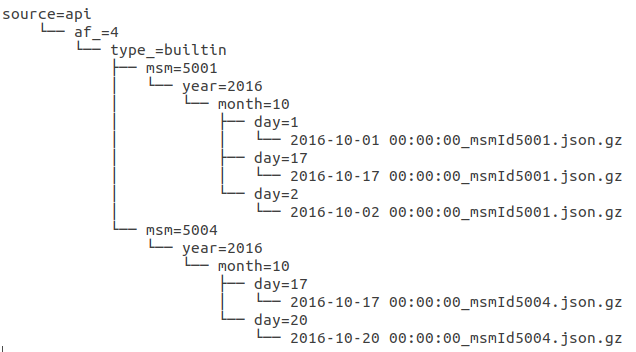
\includegraphics[width=0.6\linewidth]{illustrations/partitionnement-athena}
	\caption{L'organisation des traceroutes dans un compartiment Amazon S3}
	\label{fig:partitionnement-athena}
\end{figure}
 

\subsection{L'interrogation de données sur Amazon Athena}

L'interrogation de données présentes sur Amazon S3 via Amazon Athena est effectué avec une requête SQL. On peut décomposer une requête SQL en trois parties principales:

\begin{description}
\item[Les données sollicitées] Ça peut être une colonne ou bien bien une colonne transformée suite à l'application d'une ou de plusieurs fonctions de Presto.
\item[Les partitions de données concernées] La requête SQL est paramétrée de sorte à limiter les données à analyser sur Amazon S3. 
\item[Les paramètres appliqués sur les colonnes] La requête SQL doit filtrer les données suivant les conditions sur les colonnes de la table.
\end{description}
En pratique, nous avons créé la requête SQL reprise dans la Figure \ref{fig:sqlrequestathena}. 


Pour les données sollicitées, ce sont les trois colonnes \textit{prb\_id}, \textit{from}, \textit{msm\_id} (ligne $2$)et la liste de saut (\textit{hops})obtenue après quelques vérifications (lignes $3$ à $9$). A la ligne $10$, c'est la table créée pour les traceroutes (voir les détails de la table dans \ref{createAthenaTable}). Les traceroutes à analyser sont ceux obtenus en vérifiant les conditions dans la ligne  $12$ et $13$. C'est à dire, Athena va regarder les traceroutes qui se trouvent dans les sous dossiers year=2016\\month=10\\day=21 qui se trouvent aussi dans les deux dossiers msm=5001 et msm=5004. Ce que revient à chercher les traceroutes dans les deux endroits suivants:

\begin{lstlisting}[basicstyle= \footnotesize]
s3://ripeatlasdata/traceroute/source=api/af_=4/type_=builtin/msm=5001/year=2016/month=10/day=21

s3://ripeatlasdata/traceroute/source=api/af_=4/type_=builtin/msm=5004/year=2016/month=10/day=21
\end{lstlisting}



\begin{figure}[H]
	\centering
	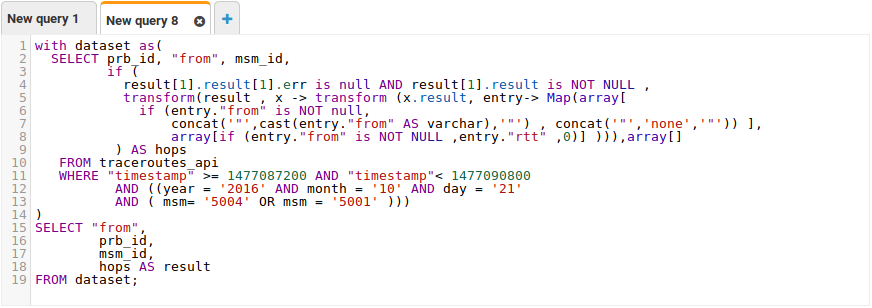
\includegraphics[width=1\linewidth]{illustrations/sqlRequestAthena.png}
	\caption{Une exemple d'une requête SQL sur Amazon Athena}
	\label{fig:sqlrequestathena}
\end{figure}


